

\tikzset{every picture/.style={line width=0.75pt}} %set default line width to 0.75pt        

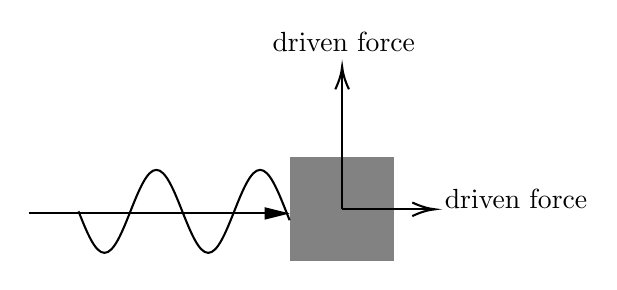
\begin{tikzpicture}[x=0.75pt,y=0.75pt,yscale=-1,xscale=1]
%uncomment if require: \path (0,300); %set diagram left start at 0, and has height of 300

%Shape: Square [id:dp3090014182756575] 
\draw  [draw opacity=0][fill={rgb, 255:red, 0; green, 0; blue, 0 }  ,fill opacity=0.49 ] (293,109) -- (343,109) -- (343,159) -- (293,159) -- cycle ;
%Straight Lines [id:da7428621460287568] 
\draw    (167,136) -- (290.71,136) ;
\draw [shift={(292.71,136)}, rotate = 180] [fill={rgb, 255:red, 0; green, 0; blue, 0 }  ][line width=0.08]  [draw opacity=0] (12,-3) -- (0,0) -- (12,3) -- cycle    ;
%Shape: Wave [id:dp7730207353336462] 
\draw   (191,135) .. controls (195.08,145.25) and (198.98,155) .. (203.5,155) .. controls (208.02,155) and (211.92,145.25) .. (216,135) .. controls (220.08,124.75) and (223.98,115) .. (228.5,115) .. controls (233.02,115) and (236.92,124.75) .. (241,135) .. controls (245.08,145.25) and (248.98,155) .. (253.5,155) .. controls (258.02,155) and (261.92,145.25) .. (266,135) .. controls (270.08,124.75) and (273.98,115) .. (278.5,115) .. controls (283.02,115) and (286.92,124.75) .. (291,135) .. controls (291.57,136.44) and (292.14,137.86) .. (292.71,139.25) ;
%Straight Lines [id:da013348464261670578] 
\draw    (318,134) -- (318,67.26) ;
\draw [shift={(318,65.26)}, rotate = 450] [color={rgb, 255:red, 0; green, 0; blue, 0 }  ][line width=0.75]    (10.93,-3.29) .. controls (6.95,-1.4) and (3.31,-0.3) .. (0,0) .. controls (3.31,0.3) and (6.95,1.4) .. (10.93,3.29)   ;
%Straight Lines [id:da44690222881601005] 
\draw    (318,134) -- (360.71,134) ;
\draw [shift={(362.71,134)}, rotate = 180] [color={rgb, 255:red, 0; green, 0; blue, 0 }  ][line width=0.75]    (10.93,-3.29) .. controls (6.95,-1.4) and (3.31,-0.3) .. (0,0) .. controls (3.31,0.3) and (6.95,1.4) .. (10.93,3.29)   ;

% Text Node
\draw (283,47) node [anchor=north west][inner sep=0.75pt]   [align=left] {driven force};
% Text Node
\draw (366,123) node [anchor=north west][inner sep=0.75pt]   [align=left] {driven force};


\end{tikzpicture}
